\chapter{Results} \label{results}
This chapter introduces the results of the study. Two classes of factors affecting experimentation in organisations were identified in the analysis process: factors that have an effect on experimentation behaviour of an individual and how experimentation affects an individual. These two classes are further divided into categories and subcategories described in this chapter. 

\section{Factors affecting experimentation behaviour of an employee}
A suitable context for experimenting was defined by the interviewees through interviews, and several factors were identified that affect in a way or another on experimentation behaviour of an employee in an organisation. In the analysis process, five different categories were formed of factors affecting experimentation. Table \ref{tbl:class1} summarises those categories and subcategories. 

\begin{figure}[!H]
\vspace{-20pt}
\hspace{-25pt}
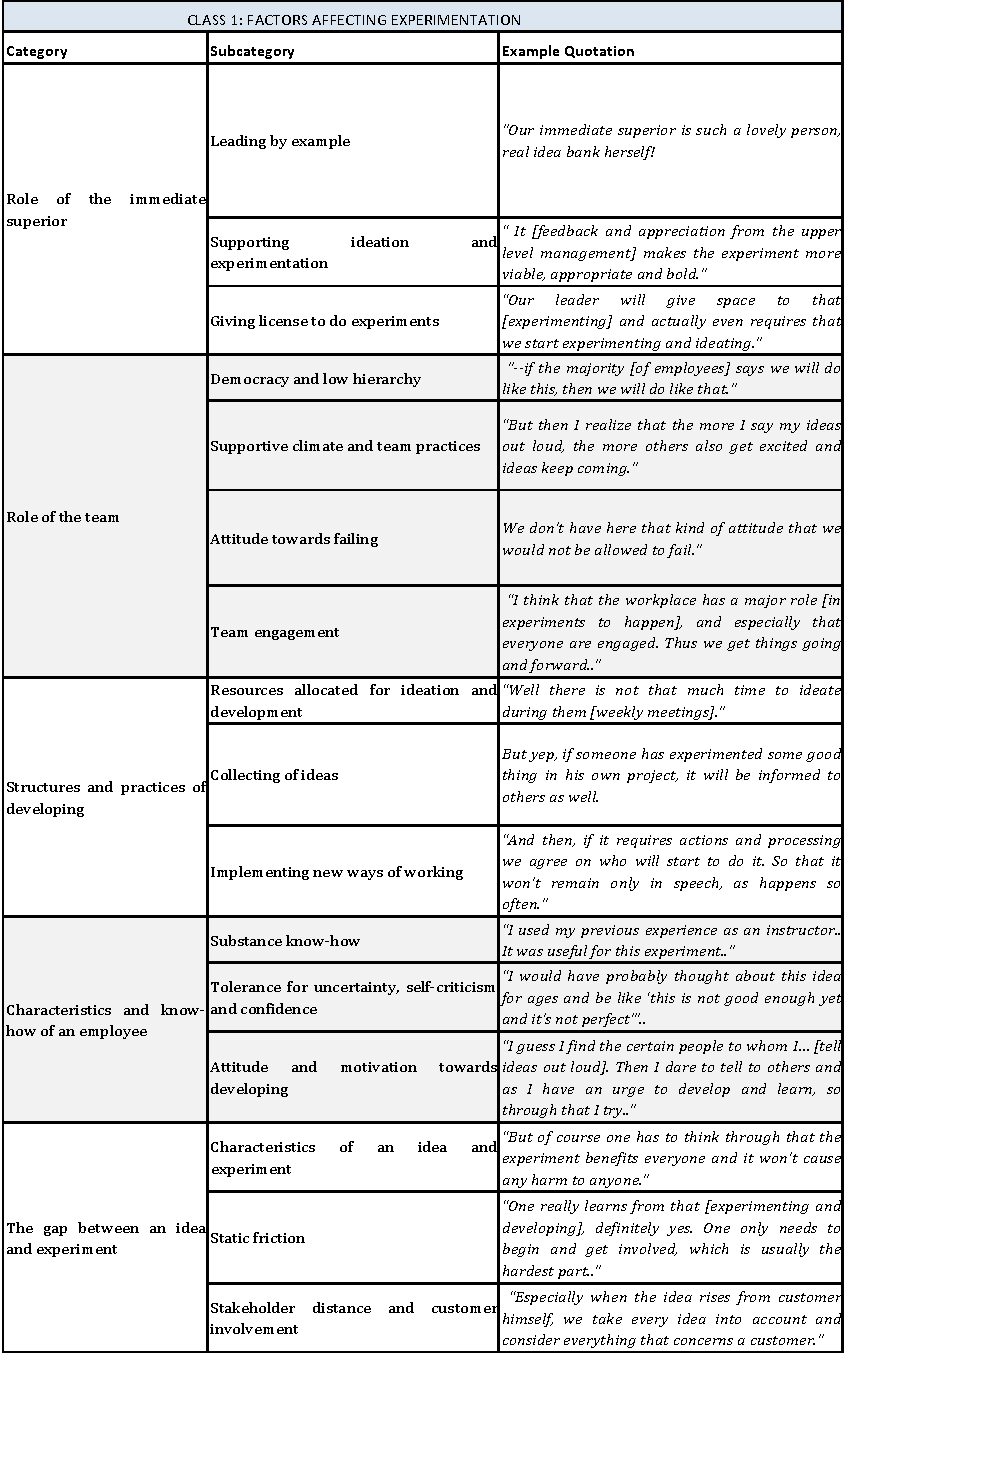
\includegraphics{class1.pdf}
\vspace{-80pt}
\caption{Factors affecting experimentation in organisations, Class 1: Factors affecting experimentation behaviour of an individual}
\label{tbl:class1}
\end{figure}

The experimentation process consists of ideating, planning an experiment and conducting the experiment as well as reflecting and learning from it in order to start the iterative experimentation process. Factors affecting these phases were identified from the data. 

\subsection{Role of the immediate superior}
Different kind of leadership behaviour that affects experimenting was recognised from the data. This category consists of actions an immediate superior can perform in order to encourage or discourage experimentation. Three main themes were recognised from the data, which are presented as subcategories Leading by example, Supporting ideation and experimentation and Giving license to do experiments.

\subsubsection{Leading by example}

According to the study attitude and actions of an immediate superior towards developing are important factors for the organisational unit as a whole. Interviewees claimed that experiments rarely happen if the immediate superior is not involved in the experimentation process and his attitude towards new ideas and developing is passive or negative. 

As interviewee 5 noted, especially when the work environment is passive towards developing and experiments, immediate superiors should act as role models and by own example create a trustworthy environment where employees can ideate and conduct experiments without fearing failure. Especially in a situation where an employee lacks support from colleagues for his idea and leading to disappointment, immediate superior can lead by example and join in the experiment in order it to occur and encourage the whole team to conduct experiments.
   
\begin{quote}
``Often they get shut down, new ideas, which is very sad, then I do not feel like even trying anymore, and in this point the leader is required. That he joins and says that now we will try this.. then it will succeed, but if it is only among colleagues, they [experiments] usually do not happen.'' [Interviewee 5]
\end{quote}
\begin{quote}
 ``Our immediate superior is such a lovely person, real idea bank herself! -- Luckily she is very development-oriented.. I mean it is nice that she does not stick to routines either.'' [Interviewee 11]
\end{quote}
Altogether, experiments are more likely to happen in workplace when immediate superior leads by example in ideating and conducting experiments himself, as can be seen in the comment above from interviewee 11.

\subsubsection{Supporting ideation and experimentation}

According to the study immediate superior's support and encouragement towards experimenting was experienced highly important in order experiments and ideation to occur among employees. Interviewees reported how the support from the immediate superior gives freedom to try out new practices, be creative and ideate together. This can be recognised from the comment of interviewee 14. Support from the immediate superior also encourages an employee to test ones limits, utilise one's working experience and abilities. 
\begin{quote}
 ``Both the immediate superior and the nurse in charge supported right away when they knew I am good at handwork, so they told me to use it as much as possible and experiment with customers.. and they told everyone the same.''[Interviewee 14]
\end{quote}
The immediate superior of an employee acts also as a bridge between the employees and upper level management bringing ideas from the organisation unit to upper levels. Few interviewees reported their immediate superior being extremely supporting and fighting for employees' ideas. According to interviewees, these superiors received support from upper level management as well. 
\begin{quote}
 ``And if we talk about even bigger experiments, so that we have to ask from upper level management, she [immediate superior] usually conveys our ideas further. So we get quite well support from there as well and it is only rarely when some idea is being shut down right away.'' [Interviewee 10]
\end{quote}
In most occasions where interviewees experienced support and encouragement towards experimentation, an immediate superior was himself very keen to developing, trying out new practices and experimentation-driven approach in work.   
\begin{quote}
``It [feedback and appreciation from the upper level management] makes the experiment more viable, appropriate and bold.'' [Interviewee 3]
\end{quote}
According to the study some immediate superiors show appreciation and support by noticing and rewarding conducted experimentations or successful ideas. This gives employees feeling that the experimentation and their work is meaningful and is thus likely to encourage experimenting behaviour. Interviewee 3 states above, how the experimentation becomes bigger through appreciation and support. 

\subsubsection{Giving licenses to do experiments}
However, immediate superior can not only encourage and support his employees in ideation and experimenting with words, he also has to allocate and allow resources for experimentation to happen. Thus, immediate superior is responsible for creating both environment and tools where experimenting is possible and resources are allocated for it. Many similar comments like interviewee 14 states below were recognised from the data. 
\begin{quote}
``Experimenting is possible exactly because the management is positive towards things like that. It has direct influence.. and that I can buy equipment I need and I get a possibility to organize new kind of activities and they don't resist it..'' [Interviewee 14]
\end{quote}
Important part of allowing experiments and giving license to conduct them is allowing them to fail. If failing when trying something new is considered punishable or the goals are exaggerated, it is likely to discourage employees to conduct experiments. In contrary, one interviewee described how his immediate superior gave license to do one experiment and promised to uphold an employee if some negative feedback or results occur from it. 

Furthermore, immediate superiors may even demand developing and doing experiments by explicitly requesting creative and innovative solutions, as can be seen in the comment of interviewee 1. 
\begin{quote}
``She [immediate superior] will give space to that [experimenting] and actually even requires that we start experimenting and ideating. So, that is the idea of all these projects, to be able to create new ways of doing things.'' [Interviewee 1]
\end{quote}
However, in some units there was a clear contradiction between the request of experiments and the resources allocated for ideation and experimentation. Again, in few units immediate superiors had taken this into account and provided time and resources for experimentation behaviour. 

Furthermore, as interviewee 8 noted, an essential part of experimenting is it being voluntary.
\begin{quote}
``In a certain way I think that workplace should encourage [to do experiments], but it cannot be forced..''[Interviewee 8]
\end{quote}
Freedom to ideate and participate experimenting depending on own motivation and interests as well as freedom to not do so was experienced important among interviewees. According to the study there is a significant difference whether the leader or a team encourages an employee to do experiments or if he is forced to do so. When feeling free to try out new things, ideate and develop himself and his work without asking permission constantly from different parts, an employee is more likely to perform experiments and develop his work.

\subsection{Role of the team}
Several aspects on how different characteristics of the team affects on experimenting behaviour were identified in the study. Subcategories Democracy and low hierarchy, Supportive climate and team practices towards ideating and experimenting, Attitude towards failure as well as Engagement of the team are described below.

\subsubsection{Democracy and low hierarchy}
Few interviewees reported their organisational unit having a low hierarchy making it possible to perform spontaneous experiments and tasks without asking permission and opinion from many parts. As interviewee 13 summarises, this was seen to lower the threshold and encourage experimenting.
\begin{quote}
``The low hierarchy kind of.. when you are in a big institution you always have to sort out if you can get the car of the institution and many other things, so here we don't have those kinds of things.''. [Interviewee 13]
\end{quote}
However, most of the interviewees described the democratic view being strong in addition to low hierarchy. Overly democratic environment and decision-making in a team can either courage employees to participate in ideating and in experimenting or make the environment too passive for actually performing experimentations, when one always has to have the majority on his side in order to try out new things. Interviewee 6 emphasises this in the quotation below. 
\begin{quote}
``There is a lot this kind of where you have to take the whole work group into account, big workgroup, as team work of course takes its own time so that everyone will then be, involved in developing.'' [Interviewee 6]
\end{quote}
\begin{quote}
``So there are once in a while divergent opinions. But then we discuss, and we decide together what will be done. And everyone has to kind of work like has been agreed. So if the majority [of employees] says we will do like this, then we will do like that.''[Interviewee 9]
\end{quote}
Furthermore, when ideas are turned into experiments and practice, interviewees reported team size being a factor affecting on how efficiently or well experimentation is executed. When a size of the team is large, meaning over five employees, it is more challenging to get all employees involved and hear everyone's opinion. In turn, if there are no people to reflect one's ideas with, ideas may remain in one's head and never come alive. A compromise would be needed in between these aspects. 

In addition, ways of sharing information and ideas among team is essential for experimentation. These aspects are presented more deeply in the next subcategory Supportive climate and practices. 


\subsubsection{Supportive climate and team practices}
Climate among the team seems to affect a lot on how easily ideas are said out loud in a team and experimentations performed. Factors such as open and creative atmosphere and support and positive feedback from colleagues have clearly a positive boost towards experimenting in an organisation.

A following pattern was identified from the data: Employees tend to ask opinion and permission from immediate superiors while also having a need for support from the team. Emerging ideas are preferably discussed with closest and most trustworthy colleagues in order to receive support, feedback, deeper understanding and reflection for employee's idea. Only after receiving other opinion and support are they brought to a team meeting under discussion. If the climate does not support ideating nor is safe for throwing ideas, employees are very unlikely to tell their ideas to others. 

However, interviewees, reported conversations and ideating sessions together with the whole team being important as they may encourage others to ideate and tell their suggestions out loud. In addition, one is likely to achieve better results with a team than only ideating alone. One person reported realizing it being important to say ideas out loud despite feeling insecure as it may lead to surprising outcomes and encourage more silent colleagues to participate in ideating. 

In addition, interviewees described ideas starting to grow the more they are thrown into discussion, and the heterogeneity of the team being mostly inspirational and beneficial in ideation phase. Interviewee 6 summarises the power of ideating in teams. 
\begin{quote}
``But then I realize that the more I say my ideas out loud, others also get excited and ideas keep coming. So it is worth speaking, even though sometimes one might think that I cannot be always talking, so it is good to keep on talking and others will follow..'' [Interviewee 6]
\end{quote}
\begin{quote}
``We also have few who are not that active in throwing ideas or performing and they like the routines, I guess the workplace could somehow support them in developing..'' [Interviewee 11]
\end{quote}
Furthermore, as interviewee 11 states above, team and climate should encourage and support employees to participate in ideating and experimenting in order an employee to overcome oneself and gently push towards new ways of doing things. 

\subsubsection{Attitude towards failing}
While discussion and giving and receiving feedback are essential in ideating phase, license to fail plays a major role when an actual experimentation is performed. Team being judgemental towards ideas and experiments can prevent actual learning and reflection of experimentations.  

Thus, one part of the supportive climate towards ideating and experimenting is the attitude towards the results of experiments. Seems that if the climate in the team allows failing and does not take it too seriously, ideation and experimentation occur more often than if a team is afraid of failing. Quote from interviewee 1 describes attitude in their unit towards failing, several similar comments about trying again together and allowing failure were recognised from the data. 
\begin{quote}
``Well no one will get punished or be thrown tomatoes at [if an experimentation fails].. I think we go through the idea and experiment, and try another way.. We do not have here that kind of attitude that we would not be allowed to fail.'' [Interviewee 1]
\end{quote}

Most interviewees described the team being very supportive and attitude towards failure positive and constructive. They rather see failure as an opportunity or a learning point. Some interviewees described going through a failed idea or experiment among team in order to find an alternative way to test the idea. This attitude seemed to help the team in experimentation behaviour. 
\begin{quote}
``I think the team reacts very well to it [failing], kind of laughing and saying that these things happen and are part of this work.''[Interviewee 6]
\end{quote}
As interviewee 6 described above, humor was also described as an important way to cope with failures and to support team members in their work. 

\subsubsection{Team engagement}
While most of the interviewees reported the workplace environment being very democratic and discursive, they described a high possibility that experimentations are not likely to happen if everyone in the team is not involved and engaged to turning idea into an experiment. Comment from interviewee 9 describes this further.
\begin{quote}
 ``I think that the workplace has a major role [in experiments to happen], and especially that everyone are engaged. Thus we get things going and forward..'' [Interviewee 9]
\end{quote}
Interviewees reported feeling frustrated when realizing how all colleagues who are involved in the experiment are not engaging to it, thus preventing an experiment to happen and get relevant feedback from it. One way to motivate and engage the team was found from the data and is presented in the subcategory Characteristics of the idea and experiment under category Gap between idea and experiment. Furthermore, the team is more likely to engage to an experiment when the purpose of the experiment is clear and shared goal exists.  

In addition, as interviewee 14 mentioned below, in order to foster the engagement of employees and the team, a team could encourage new employees to utilize their own strengths and ideate courageously. Few interviewees described their colleagues being highly supportive towards one's special abilities and skills, and encouraging everyone to use them freely at work. This was experienced as improving the level of engagement towards developing and ideating.
\begin{quote}
``Every employee is allowed to use those resources and creativity that one has in the job..'' [Interviewee 14]
\end{quote}
Shared and understandable goal for an experiment forms a strong basis for idea turning into an experiment. According to the interviewees employees and the whole team is more likely to engage to the experiment if they understand in a deeper level the reason and goal for experiment. Thus, as following quote from interviewee 11 suggests, employees are more easily involved if the goal for the experiment can be clearly justified. 
\begin{quote}
``There we had a clear goal, that somehow we just have to make it work. Then we just processed it and nothing special, it was that kind [of an experiment] with a clear goal, yep.'' [Interviewee 11]
\end{quote}

\subsection{Structures and practices of developing}
According to the study, various organisational structures and daily practices can support or prevent experimentation and ideation. First of all, the meaning of Resources allocated for ideation and development is presented. Secondly, seems that most of the units interviewed lack of systematic way for Collecting ideas, resulting to inefficient way of developing. In addition, in order the change actually happen Implementing new ways of working has to be considered. 

\subsubsection{Resources allocated for ideation and development}
Only little or no solid structure for ideation and developing was found in organisational units throughout the analyzing process. Interviewees described ideas usually emerging when a problem is encountered and an alternative way of performing is needed. In some occasions, ideas emerge accidentally  in conversations with colleagues, team meetings and rarely in meetings where developing is a specific agenda. Rather than developing purposefully interviewees described their daily work as practice-driven. 
\begin{quote}
``It can be that some person suddenly brings a good idea or then we have a specific team meeting, where the idea is to develop something. Or then some new idea might come up in some bigger meeting by accident..''[Interviewee 4]
\end{quote}
No time allocated for ideation and development of ideas leads easily to a situation where routines are repeated. In every interview time came to prominence as a lacking factor preventing ideation and experimentation from happening. Interviewees described the usual way for telling ideas and planning experiments being weekly or monthly team meetings with colleagues. As interviewee 1 states, however, these meeting usually did not include specific time for ideating and developing, more did they concentrate on routine issues. Most of the interviewees wished to have more time for ideation, developing and implementing experimentation-driven development to daily routine. Only one interviewee described having enough time for ideating. 
\begin{quote}
``Well there is not that much time to ideate during them [weekly meetings].'' [Interviewee 1]
\end{quote}
At present, most interviewees described how developing is not seen as a routine part of work but as an additional part that needs time allocated for it. Few interviewees, like interviewee 2 above, experienced experimenting challenge as a refreshing way to remind the workplace of challenging conventions and the daily routine and even thought about it becoming an annual tradition. The interviewees described that reflection is more likely to happen in between different projects and in project-type work, and when the emphasis of the work is not project-like, developing is more likely to be put aside. 
\begin{quote}
``Once a year could be kind of more intensive period or so, maybe it would maintain that no one would be too routinized. And especially in these projects that last long, so long that they are actually no longer projects, it could be quite good..'' [Interviewee 2]
\end{quote}
One interviewee described peer resources being used only little in order to exchange ideas and best practices. He suggested more meetings and ideation sessions with peer colleagues throughout Finland or even abroad in order to exchange opinions, gain perspective and find fresh, new and valuable practices to daily routine work. 
\begin{quote}
``Well, I guess the workload of some people is already so huge, causing also that people start doing things in the same way, continuing the routine..'' [Interviewee 5]
\end{quote}
Quote below from interviewee 5 clarifies how heavy workload can lead to repeating routine way of working. Sick leaves, heavy workload and hectic pace of work all affect on motivation and possibilities for developing and ideating. Furthermore, resources such as money were mentioned during the interviews as a lacking factor preventing experimentation. 

In turn, interviewees who described successful experiments said an essential factor for the success was that all the resources such as people, equipment and time were at the right place at the same time and there where no hindrances preventing experiment. Thus seems that an aspiration for using resources efficiently is essential. 

\subsubsection{Collecting of ideas}
In addition to rather usual communication problems in an organisation, the interviewed units lacked a working system for collecting ideas or feedback from experiments. The need for collecting ideas systematically was however recognised, as interviewee 5 emphasises.. Interviewees report daily work and notions in a system called DomaCare, and all employees are responsible for reading both those notes as well as ones from team meetings. 
\begin{quote}
``So of course during this one year we have had all kinds of good and bad ideas, and they are not documented.. So.. It could have been a good idea to document them..'' [Interviewee 5]
\end{quote}
However, DomaCare is not a place for new ideas, and people not reading what has been written in DomaCare remain a problem. Information is exchanged when work shift ends and other begins. Interviewees described through conversation essential information is likely to come up, thus telling about ideas and experiments should be obvious. For instance a situation where something has been already experimented before, but no reporting was made; without conversation the same experiment may be performed again, resulting to waisting time and other resources.In turn, interviewee 4 describes how successful experimentations are shared with a team. 
\begin{quote}
``But yep, if someone has experimented some good thing in his own project, it will be informed to others as well. Like hey this is what we have and this is worth experimenting.We have regular team meetings where information is shared widely, so we now what others are doing.''[Interviewee 4]
\end{quote}
The interviewees regarding reporting of experiments brought up somewhat contradictory points of views. Some interviewees claimed positive experiments being more under discussion and reporting, whereas others emphasized how failed ones raise more conversation and opinions among colleagues. However, clear and systematic practice for this was not recognised, and seems the most popular mode to share knowledge remains face-to-face conversations.

\subsubsection{Implementing new ways of working}
After experimentation being successfully executed, interviewees described the major difficulty lying behind the implementation process. Interviewees reported insightful experiments and solutions that would be important to implement in the daily routine. However, seems that structures and practices easily prevent implementing new ways of performing. For instance, new practice taking more resources in the implementation phase yet being more efficient and helpful in the long run, is more likely to be turned down and workplace sticking to old routines. 

Interviewee 5 describes one way how interviewees have tried to ease the difficulty of implementing new way of working; Deciding person or people who are in charge of the change to happen in the beginning. 
\begin{quote}
``And then, if it requires actions and processing we agree on who will start to do it. So that it will not remain only in speech, as happens so often.'' [Interviewee 5]
\end{quote}
Same phenomena and strong synergy to the difficulty of the implementation of a new routine is described in the subcategory Static Friction, which can be found under a category Gap between an idea and experiment. 

\subsection{Characteristics and know-how of an employee}
In the analysis process occurred that individual characteristics and knowledge of an employee could assist experimentation-driven approach in development as well as prevent experimentation from happening. In this category these factors are presented in three subcategories. Substance know-how explains the extent to which prior working experience can both encourage experimenting and in turn lead to repeating routines and resisting change. Individual characteristics consist of the factors how tolerance of uncertainty, employee's self-criticism and confidence affect experimenting. Attitude towards development of an employee also has a major impact on experimenting behaviour, whether an employee considers developing part of the work or not and whether he is open for new ideas and breaking routines. 

\subsubsection{Substance know-how}
According to the study prior work experience affects on the threshold for experimenting especially when experiments concern customers. Through substance knowledge an employee can gain wide understanding of the field, customer and ways of working, which can assist experimenting by adding the courage of the employee to perform an experiment. Knowing the customer, stakeholder and field of work are likely to add self-esteem and employees self-image as workers. 

Those interviewees who were recently graduated and had little previous working experience described it taking time to get to know the routines and the organisational culture as well as customers before actually being ready to suggest anything new or perform experiments. They felt easily insecure and described it important listening to more experienced colleagues and asking their opinion about new ideas before experimenting. When asked what is needed from an employee to begin with performing experiments the interviewees reported experience and knowing what to do being essential. Interviewee 6 describes the meaning of work experience to the ability to be creative and ideate. 
\begin{quote}
``In the beginning it of course took some time for me to learn the basics of the work, so maybe my own creativity and ability to ideate now grows with the experience of this work..'' [Interviewee 6]
\end{quote}
Furthermore, interviewees who had several years working experience, like interviewee 14 below, considered as a positive factor that they were able to combine previous experience to present work environment and customers. Working with same customer segment in different units gives perspective of what kind of ideas can be easily experimented and what may need more effort and resources. 
\begin{quote}
``I used my previous experience as an instructor.. It was useful for this experiment..'' [Interviewee 14]
\end{quote}
In addition, working many years with same customers leads to a high mutual trust between an employee and a customer. This again eases suggesting new ideas and performing experiments with customers. 
\begin{quote}
 ``I think there is the gained trust that has grown during this working journey. So that.. I think there is no resident [customer] who could not join doing these [experiments].''[Interviewee 7]
\end{quote}
In turn, many years of working experience from the same field and similar customer segments can also lead to repeating familiar routines and resisting change. Few interviewees described being essential that there are also newly graduated people or trainees with no prior experience in order to more clearly perceive unnecessary routines and bring new and fresh ideas into workplace. 

\subsubsection{Tolerance for uncertainty, self-criticism and confidence}
According to the study, the way an employee tolerates uncertainty may have high impact on the experimentation behaviour. When asking how interviewees feel experimentation-driven approach affecting on their work few of them described the difficulty lying in the feeling of uncertainty and incompleteness. Where some experienced uncertainty and incompleteness as threats and anxious factors in work, others emphasized those being factors that make working interesting. Interviewee 4 emphasises the ability to tolerate uncertainty and own failures.
\begin{quote}
``On the other hand it [uncertainty] is richness in work, so that one will not get too routinised. But of course one has to tolerate the uncertainty and has to tolerate your own failures, like 'ok, this time I chose wrong'..''[Interviewee 4]
\end{quote}
Furthermore, high level of self-criticism may prevent an employee from conducting experiments. Few interviewees described how they usually like to spend a lot of time in planning and refining a new idea before trying it in action. However, through the deadline and the pressure of experimentation challenge they were able to lower the level of self-criticism and try something incomplete. Interviewees learnt surprising facts already from the small experiment, and were overall satisfied experimenting even though they were not totally satisfied with the idea or experiment. As interviewee 4 states, a trifle of pressure can boost experimenting.
\begin{quote}
``I would have probably thought about this idea for ages and be like this is not good enough yet and it is not perfect''. [Interviewee 4]
\end{quote}
Self-criticism is also likely to prevent an employee saying ideas out loud. An employee may feel insecure and that his idea is actually poor and not worth sharing. An employee may even feel scared of team member shooting down his idea. As mentioned in the category Role of the team, a team can support its members to lower the level of self-criticism and encourage in ideating and experimenting. 

In turn, some interviewees described throwing also wild ideas among a team, as they may lead to something good and encourage others in ideating as well, as interviewee 6 points out. Their level of self-criticism was considerably lower and confidence higher than the ones who were not that enthusiastic in sharing ideas out loud. According to interviewee 11, personality affects on employee's opinion on failure. 
\begin{quote}
 ``I sometimes say out loud stupid ideas as well.. It's that sometimes stupid ideas can lead to anything.'' [Interviewee 6]
\end{quote}
\begin{quote}
``I do think it depends on a personality. One has to be ready for failing and not fear it.'' [Interviewee 11]
\end{quote}
Even though saying ideas out loud requires courage and confidence, it can be learnt by experience. According to the study the employees who had more previous work experience were also the ones who were more confident in telling ideas out loud and conducting experiments without fearing failure.

\subsubsection{Attitude and motivation towards developing}
According to the interviews attitude towards developing affects on experimentation behaviour. If an employee considers developing and learning new things important and part of the work, he is more likely to reframe failures as opportunities, be resilient in developing and find alternative ways of doing things that needs change. 

If a team is not supporting employee's idea and experimenting, an employee has to have motivation to try again and find another way. For instance, if the team is likely to be negative towards new ideas, interviewees described telling their ideas first to a trusted colleague. After the support from a close colleague an employee feels he has enough confidence to tell the idea to the whole team. Interviewee 9 describes this phenomena in the quote below. 
\begin{quote}
``I guess I find the certain people to whom I [tell ideas out loud]. Then I dare to tell to others and as I have an urge to develop and learn, so through that I try..'' [Interviewee 9]
\end{quote}
Thus, the meaning of an employee's motivation and attitude towards developing and learning is remarkable. In one experiment an employee ideated and prepared a prototype during his leisure time and during the process learnt new skills he had not known before. His motivation was so high it took him less than two weeks from the idea to actual prototype and first tests with customers. In turn, if an employee is not excited about learning new things, enjoys routines and prefers little change, he most likely will not be the first one to ideate or conduct experiments. As interviewee 14 states, developing requires action from an individual. 
\begin{quote}
 ``It [developing] requires activity from oneself and that an employee is willing to act and knows what he wants.'' [Interviewee 14]
\end{quote}
Furhtermore, in order ideation and experimentation to begin an employee has to be motivated and have the resilient attitude towards failing and learning from it. 

\subsection{The gap between an idea and experiment}
According to the study an idea that is said out loud in an organisation is not always easily developed into an experiment or a new routine; there seems to be a gap between an idea and experiment.  In this category factors related to idea and people involved that are critical for experimentation to happen are presented.

Interviewees reported several factors that need to be taken into account when moving from an idea to experiment, and those factors are here divided into three subcategories. Characteristics of an idea and experiment focus on how the size, riskiness and relevance of the idea and experiment can prevent or support an experiment to happen. In addition, a phenomenon called Static friction was recognised in the study, meaning that even though employees are excited about ideating and experimenting in the beginning, for some reason experiments still do not take place. Stakeholder distance and customer involvement consists of the importance of stakeholder and customer opinion on the experiment as well as mutual trust between different parties that experiment concerns. 

\subsubsection{Characteristics of an idea and experiment}
Characteristics of an idea seem to have an impact on whether or not it is experimented. For instance, the simpler and more concrete the idea is, the more likely it is to be experimented. Experimentation seems to help in making abstract ideas into concrete things and reflect the problem more clearly. However, even though the idea gains positive feedback among workplace, it still might not be experimented. The more resources, planning and opinions from different parts are needed in experiment and the more complex it feels among participants, the more likely it is to remain in ideation phase and not evolved into an experiment.  Interviewee 1 describes below why an idea actually turned into an actual experiment.
\begin{quote}
``It was as concrete thing as possible, that did not take too much.. or more 
negotiation with different parts..'' [Interviewee 1]
\end{quote}
The risk level of an idea affects on the bridge between throwing ideas and actually experimenting. When talking about performed experimentations interviewees, like interviewee 10 below, described the first ideas behind them being easy and simple, and especially possible to experiment with a low risk of anything bad to happen to customers or people involved in the experiment. In addition, interviewees reported that suitable experiments take into account the characteristics and possible limitations of the team or experiment. 
\begin{quote}
``But of course one has to think through that the experiment benefits everyone and it will not cause any harm to anyone.''[Interviewee 10]
\end{quote}
In addition, relevance and importance of an idea and the problem it attempts to solve are essential for the gap between an idea and experiment. Be the problem widely recognised among workplace, an attempt to experiment something new is rather likely to get support and engagement from colleagues and stakeholders. Likewise, according to the study if employees do not consider an idea important, and are not motivated to perform it, the idea will presumably be shut down by colleagues rather than considered from different perspectives or experimented nevertheless. 

\subsubsection{Static friction}
Static friction in organisational environment came to prominence in the study.  Static friction here means a workplace, despite of eagerness towards new ideas and ideating, sticking to the routines and not being able to act in a different way and experimenting new ways of working. Employees are likely to get excited of ideas and even ideate eagerly together as a team, yet when it comes to implementation and actually performing experiments or do something differently, employees are no longer willing to take responsibility or be that excited about the idea. Interviewee 8 describes the phenomenon.
\begin{quote}
``I think we are always so excited about everything, but when we start going through details and who will actually take charge of this and who will be involved, then I think we are no longer that excited..'' [Interviewee 8]
\end{quote}
In turn, as interviewee 3 put it, few interviewees described a situation where little or no static friction is recognised. Common factor to these descriptions is that when coming up with an idea, employees begin right away going through different possibilities and actions on how to perform an experiment or implement the idea and actually proceed with them. Yet in the study descriptions about static friction were in majority. 
\begin{quote}
``I start quickly ideating where I can contact next [in order to make perform the experiment or gain a certain goal]..'' [Interviewee 3]
\end{quote}
\begin{quote}
``One really learns from that [experimenting and developing], definitely yes. One only needs to begin and get involved, which is usually the hard part..'' [Interviewee 5]
\end{quote}
Even though interviewees emphasized learning and experimenting new ideas being essential for work, lot of resistance and inactivity occurred when actual experimenting was supposed to happen. Interviewees described even being surprised how after all the enthusiasm towards experimenting, no one was willing to take the lead and the experiment was never performed. Interviewees supposed and admitted that at times it feels too exhausting and difficult to break routines and it is easier to continue performing tasks as is used to. 


\subsubsection{Stakeholder distance and customer involvement}
According to the study the relevance and closeness of the idea to the customer enhances the engagement for experiment of employees. According to interviewee 7, the need for a change rising from a customer, improves the likelihood of the idea taken seriously and experimented. The same applies when a clear need to try something new is present. This is usually faced as a problem in present way of working, yet it can also be an attempt to improve the quality of customer's life or the atmosphere at the workplace.  
\begin{quote}
 ``Especially when the idea rises from customer himself, we take every idea into account and consider everything that concerns a customer.'' [Interviewee 7]
\end{quote}
In this specific working field experimentation that concerns customers needs permission usually from both customer and relatives. According to the study this is occasionally a challenging network to deal with, as the requirements and wishes from customers and stakeholders may be highly contradictory. Yet, worthy ideas also rise from relatives as well as relevant information of what has already been experimented with the customers and what was learnt from that. Interviewee 10 describes this phenomenon. 
\begin{quote}
``So relatives play a very central role in our customers' lives, and almost everything is still discussed and checked with them and ask for support from them, like can we do this. And some very good ideas may also rise from them. Or then it can be like 'Oh no, this has been experimented for 15 years now, and it doesn't work, so you should not start doing this.'.. So we have to remember that there is the network outside this workplace that is usually also involved in these experiments.'' [Interviewee 10]
\end{quote}
Mutual trust between people involved in experiments is needed. Interviewees described mutual trust being a relevant part of experimenting, and experienced the trust especially among customers and stakeholders as highly important factor in order experiments to happen. 

\section{How experimenting affects an individual}
In the analysis process another class was identified: the effects experimenting has on individual. This second class and its categories are presented in figure \ref{tbl:class2}

Experimentation has an effect on employee on different levels. First of all, wide variety of emotions, such as excitement, fear of failure, disappointment and uncertainty is involved and rises up at different phases of the experimentation process. Secondly, experimenting helps an employee to learn and reflect on one's work as well as to gain process know-how of experimenting. It seems that through experimenting an employee is likely to encounter surprising outcomes that would not have been realised and learnt through planning.  

\begin{figure}[!H]
\vspace{-30pt}
\hspace{-35pt}
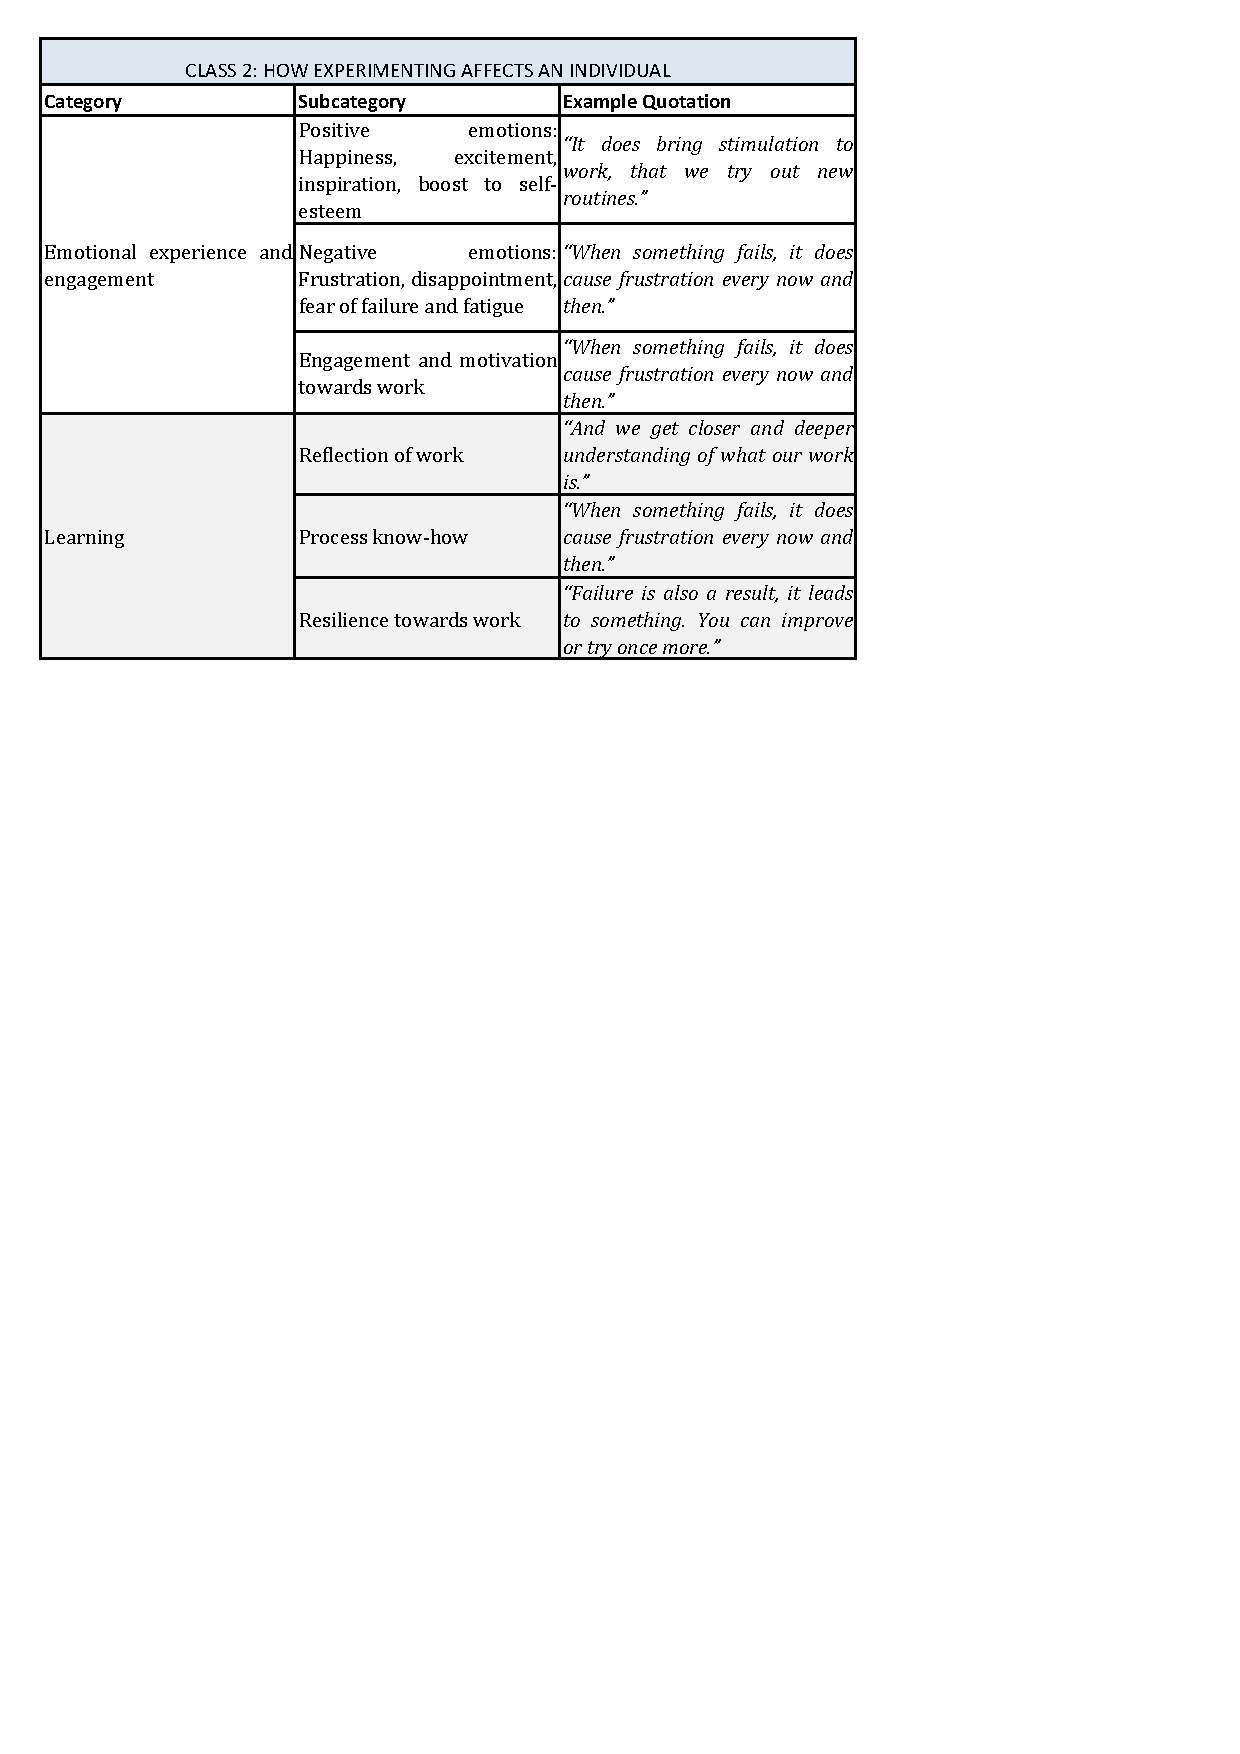
\includegraphics{class2.pdf}
\vspace{-220pt}
\hspace{-400pt}
\caption{Factors affecting experimentation in organisations, Class 2: How experimenting affects an individual}
\label{tbl:class2}
\end{figure}

\subsection{Emotional experience and engagement}
The study revealed that during the experimentation process an individual experiences wide range of emotions. Those factors are presented here in three subcategories, which are Positive emotions: Happiness, excitement, inspiration, boost to self-esteem, Negative emotions: Frustration, disappointment, fear of failure and fatigue and Engagement and motivation towards work. These subcategories are described and explained, in which part of the experimentation process they are usually faced. 

\subsubsection{Positive emotions: happiness, excitement, inspiration, boost to self-esteem}
Experimentation usually begins with ideation, and in this phase interviewees described feeling creative, happy and excited. Ideating feels inspiring when colleagues support and join the ideating and plan together how the idea could be experimented. Interviewees described being excited and happy especially when the idea was their own or they were highly involved in ideating and planning the experiment.  Furthermore, ideating as a group also felt more empowering than ideating alone and not getting support for one's ideas. 

As Interviewee 4 states, positive results of experimenting, meaning that new way of doing things works better than the previous way, is likely to raise positive emotions. Interviewees described that getting good feedback from the experiments and ideas as well as getting support from both customers and colleagues raise positive emotions and give boost to self-confidence. Furthermore, a successful experimentation encourages experimentation behaviour and ideating and was described to nourish one's creativity, as interviewee 6 emphasises.  
\begin{quote}
``If something works better than before [experimenting], you get a good feeling out of that.'' [Interviewee 4]
\end{quote}
\begin{quote}
``Experimenting nourishes creativity and ability to throw oneself to something new.'' [Interviewee 6]
\end{quote}
Among some interviewees the uncertain outcomes of experiments can also be seen as exciting and refreshing possibilities. As by experimenting new ways of performing work tasks are tested, experimenting brings exciting new aspects and challenges to routine work. Good ones tend to spread and may lead to something new and energetic and are likely to bring energy and stimulation to an employee. Interviewee 10 describes how experimentation brings stimulation to work. 
\begin{quote}
``So the experimentation kind of spreads. And I do also like routines and stuff: that things go in a certain way. But, it does bring stimulation to work, that we try out new routines.'' [Interviewee 10]
\end{quote}

\subsubsection{Negative emotions: frustration, disappointment, fear of failure and fatigue}
Among positive emotions, interviewees described encountering various uncomfortable and complicated feelings throughout the experimentation process. 

In cases where an idea of an employee gets only little or no support from the team or a manager, feelings of frustration and disappointment may occur. This phenomenon is likely to discourage employees to say their ideas out loud in the future and thus makes the level of employee's self-criticism higher. In the quote below of interviewee 14, is described the feeling of disappointment when encountering resistance from colleagues or team.
\begin{quote}
``When you are totally excited about something [idea].. for sure there comes the disappointment like what is it now, why this idea cannot go through, what is it that is so difficult in this.''[Interviewee 14]
\end{quote}
While the outcome of experimentation is usually difficult to forecast and cannot be planned in beforehand, this has an influence on emotions of an employee. Tight schedule of experimenting and little planning combined to uncertain outcomes can raise anxious emotions. Saying out loud one's ideas might feel scary as the employees feel insecure about their idea. This forces them to encounter an uncomfortable fear of failure of their idea being shot down. 

In cases where the experimentation in where all the people involved are highly excited about, does not reach the goals set for the experiment, it is likely to cause frustration, disappointment and sadness among employees. In most cases, interviewees felt failing personally when they felt that experimentation failed. Interviewees usually described experimentation as failed if it did not reach the goals set for the experiment. 

In situations where there is no specific closure for the experiment or for some reason the experimentation is not finished, interviewees described feeling disappointed. This rather typical need for getting things done is described in the quote of interviewee 5.
 \begin{quote}
``Kind of disappointment, or kind of feeling of failure..' I always want to finish what I start.. So I do not like if things are not finished..''[Interviewee 5]
\end{quote}
\begin{quote}
``In addition, it [the experiment] cannot be too big, as it easily inflates.. so I think it is better to start, no matter how great idea there was, to slightly narrow it in some certain idea and then experiment that one. As I think many times it is a major hindrance that employees have no energy when the experiment inflates too much..'' [Interviewee 8]
\end{quote}
As described in quotation above from interviewee 8, the size of an experiment has an effect on the energy level of an employee. When planned experiment is too large or complicated and tasks needed to perform it too challenging or numerous, lots of resources are consumed and the energy level of an individual is lowered causing fatigue. 

\subsubsection{Engagement and motivation towards work}
The experience of experimentation and seeing the result of experimentation is likely to encourage employees in their work.  Especially when the employees performing an experiment are satisfied with the outcomes of the experimentation, so that they consider it successful, experimenting improves the engagement and motivation of an employee towards his work. Furthermore, this encourages employees to be more creative and say out loud one's ideas as well as gives a boost to energy level.

 As mentioned in the factors affecting experimenting, receiving feedback is important part of experimentation. In the field studied, employees work in a very close interface with customers and stakeholders. Thus, positive feedback from them raised positive emotions and encouraged to continue developing. Interviewee 10 states how important the feedback from work is for engagement.
\begin{quote}
``But every time there is a good idea and it works when we try it, and we notice that it helps, of course it improves my performing in the work also in mental level. And there comes moments, with customers, when something works with them and we get positive feedback --- of course it is very important. It then makes me happy and motivates, and encourages further on. Or feedback from relatives, if we get positive feedback from them, it again encourages.'' [Interviewee 10]
\end{quote}
Overall, interviewees described they felt more engaged to their work when they were able to perform 'quick and dirty' experiments from which they get instant feedback. Ideating and new ways of performing work-related tasks through experimenting increased the meaningfulness of work and made it more interesting. In addition, through ideating and experimenting interviewees felt they have more influence on their own work.

\subsection{Learning}
Experimenting seems to have an impact on learning skills of an individual. Learning occurs in various levels, and three subcategories where learning was especially noticed were formed from the data. Reflection of work means that experimenting helps an employee to reflect ways of working and the work overall. Secondly, through experimenting an employee gains deeper understanding of experimentation process, which is here called Process know-how.  In addition, it seems that an experimentation process helps and individual to overcome anxious and insecure emotions described above, thus improving the Resilience towards work of an employee. 

\subsubsection{Reflection of work}
According to the study experimentations helped to question conventional ways of working and offered wider, more objective perspective that helped to improve the work. Some interviewees noticed the same as interviewee 2; that stopping to reflecting one's work is not and ordinary practice for an organisation and its employees. Experimentation process helped employees to reflect and make the purpose of their own work clearer, as interviewee 8 emphasises. 
\begin{quote}
``Many things are done without actually stopping to think about them more, like would there be something to improve. It might be kind of quite typical way to act for an organisation, to forget further evaluation.''[Interviewee 2]
\end{quote}
\begin{quote}
``Maybe it differs when.. you have to think, or you get to think, but let's say that you have to think some issue in a deeper level and maybe make your thoughts more structural and that you have some understanding from what you view your own work and work of others.. 'So it does give in a certain way a deeper understanding on how one is doing his work.'' [Interviewee 8]
\end{quote}
As mentioned in the factors that affect experimentation, giving and receiving feedback is relevant in experimentation-driven approach. Receiving instant feedback improves learning process of an employee and the ability to iterate, meaning that an employee can reflect the outcomes of an experiment and improve his idea for another experiment and work overall. 

Furthermore, interviewees described surprising outcomes of small experimentations they performed and said talking about experimentations as well as performing them led to new information and ideas from different parts, including colleagues, customers and stakeholders. The interviewees described learning things they most likely would not have learnt without experimenting something new. Through experiments they also got deeper contact with stakeholders such as customer's parents. Interviewee 14 describes below his relation to customers and relatives.
\begin{quote}
``The working becomes more interesting and I have clearer targets [through experimenting]. I get better in contact with customer and find new aspects as I told.. With customer's relatives we talk in a different way when I tell that I've been planning of this kind of experiment -- and then the relatives begin to tell the history of a customer..'' [Interviewee 14]
\end{quote}
In addition to experimenting making the actual core of the work clearer, in this field of work where employees work very close to customers it helped the employees, like interviewee 6, to understand and listen better their needs and become more customer-oriented.  
\begin{quote}
``Through that [an experiment] we learnt to listen more and be even more customer-oriented ''[Interviewee 6]
\end{quote}
\begin{quote}
``Seems to me that my own prejudices are best repealed by just starting to do and act. Through that also abilities are found.'' [Interviewee 3]
\end{quote}
Furthermore, according to interviewee 3, employees learnt to overcome prejudices through rapid experimenting and found hidden capabilities.

\subsubsection{Process know-how}
Factor called process know-how was recognised from the data. In this instance, process know-how means understanding of experimentation process, including the ability to ideate, plan and perform small experiments, the ability to reflect and learn from experiments and do iterations. 

Seems that process know-how of an individual improves through the experience of experimentation. Interviewees who were more familiar with vocabulary and the process of experimentation and who had done at least one experiment during the experimentation challenge were likely to reflect experiments in a deeper level than those who were not that familiar with the process and vocabulary. 

Those who had deeper understanding of experimenting process emphasized that one can learn from each experiment whether the actual goal set for the experiment is achieved or not, and those teachings are relatively important. As interviewee 12, some said the more the experiment fails, the more could be learned from it. 
\begin{quote}
``One always learns [from experiments]. It is kind of like the worse the experimentation is, the better one learns from it.''[Interviewee 12]
\end{quote}
\begin{quote}
``Failure is also a result, it leads to something. You can improve or try once more.'' [Interviewee 3]
\end{quote}
As interviewee 3 states, failure was rather seen as a result or learning point than totally failing. Those employees who had process know-how on experimenting were able to continue and learn better from each experiment, understand failures as learning objectives, process ideas and truly develop their work and challenge conventions. They reported feedback being an essential part of the work and developing, as it teaches what has to be done differently and what was successful. Interviewee 10 shows process know-how by stating the role of feedback, whether it is positive or negative. 
\begin{quote}
``Feedback is important in that essence so that one knows is it worth to continue to other experiments. So it [feedback] is always good, whether it was positive or negative, but it is always needed.''[Interviewee 10]
\end{quote}
When talking about feedback helping reflection of the experimentations, interviewees also reported discussion with colleagues being essential. Through discussion and feedback important information is exchanged and new aspects can be found and learnt. Yet, according to the study, receiving and listening to feedback requires humility and willingness to admit own faults and receive help from others.

Furthermore, essential part of process know-how is starting to perform with small experiments, prototyping with small group of customers, making a prototype as simple as possible and learning from the iterative process. Interviewees described being surprised by how fast a rough prototype can be done and how helpful it can be for work, compared to usual way of working meaning years of developing before some tool is launched for use. 
\begin{quote}
``This thing [a prototype], was welcomed so well, and actually it helped right away.. when usually these kind of tools are developed for many years before they are valid. So actually this kind of very simple system built this fast.. So it helped right away and that was a happy surprise..'' [Interviewee 1]
\end{quote}
Furthermore, a deeper perspective of process know-how affects bigger changes in an organisation. One interviewee described experimentation as a way to manage and change complex systems while smaller experiments can assist bigger changes to happen. 
\begin{quote}
``But it can be, that this kind of small experiment can help bigger changes to happen.. And I guess that's the trick in this whole thing and behind, that large things consist of several small ones and if those small ones can be fixed in several ways, it can have great impacts..'' [Interviewee 1]
\end{quote}

\subsubsection{Resilience towards work}
Even though in experimentation process an employee goes through negative emotions described earlier such as frustration, fear of failure or disappointment, experimenting helps to overcome those anxious feelings and improves resilience of an employee.  Performing experiments forces employees to turn abstract ideas into concrete, smaller and lighter steps that are easier to approach, thus making the gap between planning and experimenting smaller.  

When experimentation is experienced as important among participants or there is a real problem to be solved, employees may turn all the disappointment and frustration rising from previous experiments or abatement of the idea from colleagues or a leader into passion of performing better. This improves the capability of resilience, as interviewee 13 comments. 
\begin{quote}
``So first comes the frustration, but after that like next year we'll show them--. It may turn upside down when I get to process it in my head, like it's a bummer how badly this went, but it can be we will try it again in a bit different way and we will do it better then. This also encourages to continue..''[Interviewee 13]
\end{quote}
Choosing the right terms may have a major impact on behaviour and resilience. Experiment as a word in a way consists of failing, and according to the study, compared to failing in daily routine work, failing in an experiment is experienced rather acceptable. This leads an employee feeling less pressure for succeeding with the first try. In addition, when the effort put on the first experiment is bearable, it is easier to persistently try another way. Interviewee 11 describes below his resistance. 
\begin{quote}
``Sometimes you really feel like giving up when you no longer come up with solutions how to make something work. But still you just.. You have a small break and then you get back to business.''[Interviewee 11]
\end{quote}
Even though during ideating and experimenting negative feelings are likely to occur, the characteristics, experience and know-how of experimenting helps to overcome these emotions and turn them to resilience. Iterative process of developing, dividing a task or a problem into smaller steps and learning by doing all support the emotional struggle with self-criticism, fear of failure, insecurity and uncertainty. 
